\documentclass[12pt]{article}
\newcommand{\MyFullName}{Jon Wedaman, Jeremy Lavergne, Alex Padgett, Jeff Farris}
\newcommand{\MyLastName}{Wedaman, Lavergne, Padgett, Farris}
\renewcommand{\indent}{\hspace{0.25in}}
\RequirePackage{macroNorm}
\title{ Parallel Computing \\ Lab 3: Radix Sort }
\author{\MyFullName}
\date{ Due June 1, 2010 }
\begin{document}
\maketitle
\thispagestyle{empty}
\begin{center}
  %Description
\end{center}
\setcounter{page}{0}
\newpage

\def\thesection{\Roman{section}.}
\hfill \\
\section{ Background }

\indent Radix sort is an integer sorting algorithm that avoids comparison operations in favor of using the integers as keys in a fixed order. 
In general it features performance of $O(k N)$ where $k$ is the bit-length, and $N$ is the number of integers.

\section{ Performance Data }
\begin{center}
\begin{tabular}{ c | c }

\textbf{Implementation} & \textbf{Time} (ms) \\ \hline
Sequential & 163 \\ 
Parallel & 512 \\ 
\end{tabular}
\end{center}

\section{ Implementation Details }
\indent  Our implementation loops over the size-$n$ list $k$ times where $k$ is the number of bits, in our case $k = 32$.   
In each loop, there are two operations performed on the list.  
The first and probably most important is computing the prefix sum of the the list.  
To compute the prefix sum, we perform a parallel scan---specifically an excluding scan---over the array of integers. 
An exclusive scan means that each index $j$ in the results list is equal to the sum of all elements up to but \emph{not} including $j$.  
To use the prefix sum in the context of Radix Sort our implementation begins by examining one bit from each integer, starting with the least significant bit. 
This generates the prefix sum of the number of bits equal to 0.  
Using the generated sum, we can re-pack the array such that all of the keys with a 0 in that bit are in front of those with a 1. Thereby we preserve the original order of the list but sort the higher numbers into bins to be sorted in later iterations. 
After each digit is examined, the numbers are be in increasing order. 

\newpage
The following illustration shows how we use the prefix sum to re-pack the list:

\begin{center}
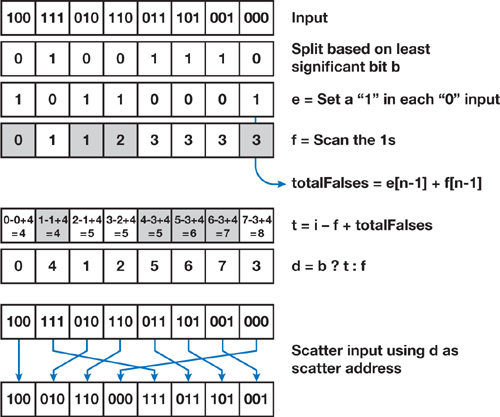
\includegraphics[width=4in]{nvidia-stuff.jpg}
\end{center}

When sorting an array of this size in a single thread block, we can use shared memory to store the lookup array referenced as $e$ in the diagram.  
Since we can't compute the prefix sum as one piece, the work must be divided amongst the 512 threads available in the thread block.  
Our implementation uses 256 threads, and assigns each thread 16 elements from which to compute a prefix sum.
Once each piece is summed, these sums are then stored in another array in global memory and each is uniformly added to each index higher in the list.  
Since we have direct access to the new addresses of the elements, we can use the prefix sum to move each element into its appropriate place in the global result list and repeat the process until all elements are sorted.

\end{document}